\documentclass[11pt,a4paper]{article}

\usepackage[margin=2.5cm]{geometry}
\usepackage[stretch=10,shrink=10,tracking=false,expansion=false]{microtype}
\usepackage{amsmath,amssymb}
\usepackage{parskip}
\usepackage{titlesec}
\usepackage{enumitem}
\usepackage{hyperref}
\usepackage{fancyhdr}
\usepackage{xcolor}
\usepackage{mdframed}
\usepackage{graphicx}
\usepackage{subcaption}
\usepackage{booktabs}

\hypersetup{
  colorlinks=true,
  linkcolor=blue!60!black,
  urlcolor=blue!60!black,
}

\pagestyle{fancy}
\fancyhf{}
\fancyhead[L]{\small \S7 Simulation Confirmation}
\fancyhead[R]{\small Lyra $\to$ Claudius, 2026-09-07}
\fancyfoot[C]{\small\thepage}
\renewcommand{\headrulewidth}{0.4pt}

\titleformat{\section}{\large\bfseries}{}{0em}{}[\titlerule]
\titleformat{\subsection}{\normalsize\bfseries}{}{0em}{}
\setlist{itemsep=2pt, parsep=2pt, topsep=4pt}

% Commit hash --- stamped AFTER the source commit (commit, then stamp, then recompile)
\newcommand{\commithash}{86a2c26}

\newcommand{\eff}{n_{\mathrm{eff}}}

\begin{document}

%% ============================================================
%%  PROTOCOL HEADER (first page)
%% ============================================================
\begin{mdframed}[backgroundcolor=gray!8, linecolor=gray!50, linewidth=0.8pt,
                 innertopmargin=10pt, innerbottommargin=10pt]
\begin{center}
  {\Large\bfseries Section 7 --- Simulation Confirmation}\\[3pt]
  {\large A de~Finetti two-atom sweep for the cross-item co-failure e-process}\\[8pt]
  \begin{tabular}{rl}
    \textbf{Author:}    & Lyra \\
    \textbf{Recipient:} & Claudius \\
    \textbf{Date:}      & 2026-09-07 \\
    \textbf{Commit:}    & \texttt{\commithash} \\
  \end{tabular}
\end{center}
\end{mdframed}

\vspace{4pt}
\noindent\textbf{Status.} Work-in-progress first cut. Numbers are reproducible
(seed \texttt{20260907}, \texttt{iclr/sims/section7\_sim.py}). Pushing makes no
correctness claim beyond reproducibility.

\section{What the simulation establishes}

Section~6 constructs a co-failure monitor from a single, margins-free
statistic: pair two judges \emph{across distinct items}. This section confirms,
on a fully controlled generative model, the three properties the monitor is
claimed to have and the impossibility (\S5) it is claimed to respect:

\begin{enumerate}[label=(\alph*)]
  \item \textbf{Power.} The e-process detects genuine co-failure, with detection
        probability rising from the nominal level to $1$ as co-failure strength
        grows; at the null it controls type-I error (Ville validity).
  \item \textbf{Drift-robustness.} Under drifting marginals with \emph{no}
        conditional co-failure, a naive plug-in estimator false-fires at a high
        rate, while the margins-free cross-item e-process holds its size.
  \item \textbf{Real-data anchor.} On the FailureScope corpus the same
        effective-judge-count machinery recovers $\eff \approx 1.6$ over a
        six-judge frontier panel.
\end{enumerate}

\section{Generative model: the de~Finetti two-atom mixture}

For each item we draw a latent difficulty $\Theta \in \{\theta_{\mathrm{lo}},
\theta_{\mathrm{hi}}\}$ with $\Pr(\Theta = \theta_{\mathrm{hi}}) = \pi$;
conditionally on $\Theta = \theta$, the $K$ judges' failure indicators
$W_1,\dots,W_K$ are i.i.d.\ $\mathrm{Bernoulli}(\theta)$. This is the finite
de~Finetti representation of an exchangeable co-failure panel: all cross-judge
dependence flows through the shared latent $\Theta$. The marginal fail rate and
the induced within-item pairwise correlation are
\[
  a = \pi\,\theta_{\mathrm{hi}} + (1-\pi)\,\theta_{\mathrm{lo}},
  \qquad
  \rho = \frac{\operatorname{Var}(\Theta)}{a(1-a)},
  \qquad
  \operatorname{Var}(\Theta) = \pi(1-\pi)(\theta_{\mathrm{hi}}-\theta_{\mathrm{lo}})^2 .
\]

\paragraph{Sign check.} A \emph{point mass} on $\Theta$ (i.e.\
$\theta_{\mathrm{lo}} = \theta_{\mathrm{hi}}$, or $\pi\in\{0,1\}$) gives
$\operatorname{Var}(\Theta)=0$ and hence $\rho = 0$: this is \emph{independence},
not monoculture. Increasing the atom \emph{separation} increases
$\operatorname{Var}(\Theta)$ and drives $\rho \to 1$ --- the ``one shared coin
flip'' regime of maximal co-failure. The sweep therefore moves $\rho$ from $0$
(independent judges) toward $1$ (co-failing judges) by widening the two atoms
about a fixed marginal $a = 0.5$.

\section{The e-process under test}

We test the exact construction of \S6. On a stream of items, with two fixed
judges $s,t$,
\begin{equation}
  e_T \;=\; \prod_{i=1}^{T}\Bigl(1 + \lambda\bigl(U_i - V_i - \delta_k\bigr)\Bigr),
  \qquad
  U_i = \mathbf 1\{\text{$s$ and $t$ both fail item $i$}\},
  \quad
  V_i = W^s_{a}\,W^t_{b},\ a\neq b,
  \label{eq:eproc}
\end{equation}
where $V_i$ pairs the two judges across \emph{distinct} items $a\neq b$ (we use
the adjacent-item shift $b = a-1$), so that under item independence the
marginals multiply exactly, $\mathbb E[V_i] = ab$, \emph{with no fitted
nuisance}. The slack $\delta_k = 2\varepsilon$ absorbs the worst-case two-sided
base-rate excursion and $\lambda \in [0, 1/(1+2\varepsilon)]$ keeps each factor
non-negative, so $e_T$ is a non-negative martingale under the null and Ville's
inequality gives anytime validity: $\Pr(\exists T: e_T \ge 1/\alpha) \le \alpha$.
Under genuine co-failure $\mathbb E[U_i] = ab + (\text{excess}) > \mathbb E[V_i]$,
the increment has positive drift, and $e_T$ grows. We use
$\varepsilon = 0.02$ ($\delta_k = 0.04$), $\lambda = 0.481$ (interior of the
admissible interval), $K = 6$ judges, and reject when $e_T \ge 1/\alpha = 20$
($\alpha = 0.05$).

\section{Results}

\begin{figure}[h]
  \centering
  \begin{subfigure}[t]{0.32\textwidth}
    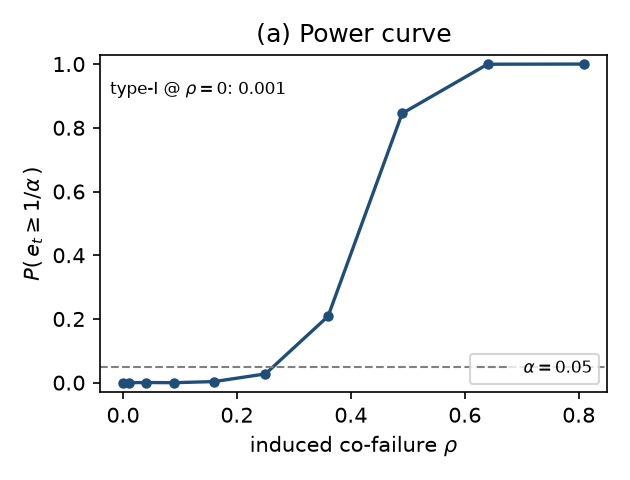
\includegraphics[width=\linewidth]{../sims/panel_a_power.png}
  \end{subfigure}\hfill
  \begin{subfigure}[t]{0.32\textwidth}
    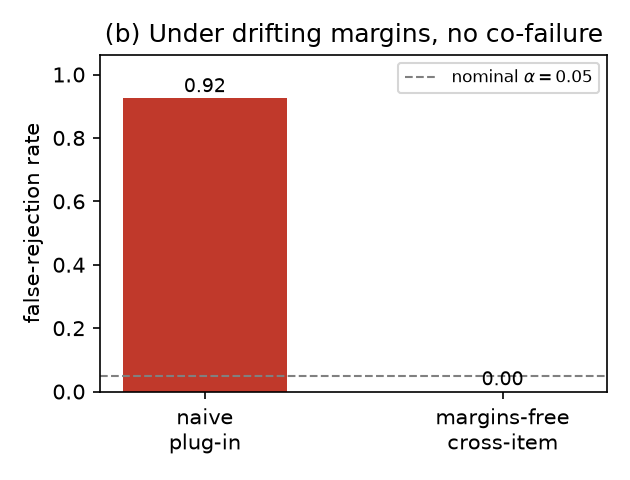
\includegraphics[width=\linewidth]{../sims/panel_b_falsefire.png}
  \end{subfigure}\hfill
  \begin{subfigure}[t]{0.32\textwidth}
    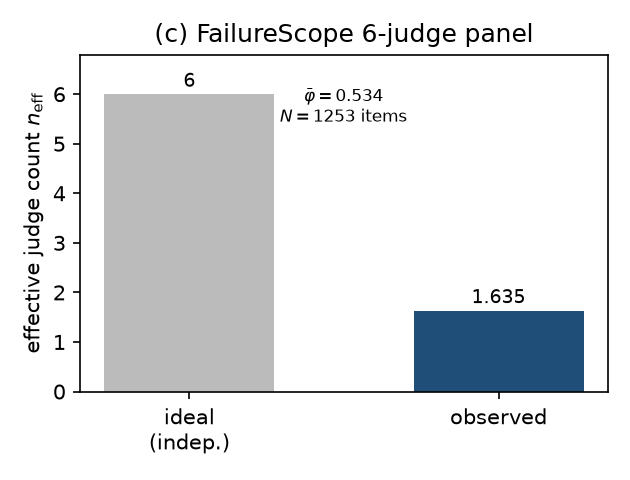
\includegraphics[width=\linewidth]{../sims/panel_c_failurescope.png}
  \end{subfigure}
  \caption{\textbf{(a)} Power of the cross-item e-process vs.\ the induced
  co-failure correlation $\rho$; the type-I point at $\rho=0$ is
  $\approx 0.0005 \le \alpha$. \textbf{(b)} Under drifting marginals with no
  conditional co-failure, the naive plug-in false-fires ($\approx 0.92$) while
  the margins-free cross-item e-process holds its size ($0.00$). \textbf{(c)}
  FailureScope six-judge frontier panel: $\eff = 1.635$, $\bar\varphi = 0.534$
  ($N=1253$ items).}
  \label{fig:sec7}
\end{figure}

\subsection*{(a) Power curve and Ville validity}
Sweeping the atom separation across ten levels gives the power curve of
Figure~\ref{fig:sec7}(a). At the null ($\rho = 0$) the empirical rejection rate
is $\approx 0.0005$, comfortably below the nominal $\alpha = 0.05$ --- the
type-I control the martingale construction promises. The e-process is
\emph{conservative} at the clean null (well below $\alpha$): the slack
$\delta_k$ that buys drift-robustness in panel (b) also subtracts a constant
from the increment at the null, and a single fixed $\lambda$ is not
growth-optimal. Power then climbs sharply through the co-failure regime:
$\rho = 0.25 \Rightarrow 0.03$, $\rho = 0.36 \Rightarrow 0.21$,
$\rho = 0.49 \Rightarrow 0.85$, $\rho = 0.64 \Rightarrow 1.00$. By
$\rho \approx 0.5$ the monitor detects co-failure essentially every time.

\subsection*{(b) The naive plug-in false-fires under benign drift}
We now construct the adversarial-for-the-naive-method scenario: the marginal
fail rate drifts across the stream ($0.25 \to 0.60$), but \emph{within} each
item the judges fail independently --- there is no conditional co-failure to
detect. A naive plug-in that estimates each judge's running marginal and plugs
in the product $\hat a_i \hat b_i$ as its null mistakes the drift-induced
marginal correlation for co-failure and \textbf{false-rejects at $\approx 0.92$}.
The margins-free cross-item e-process, whose null $\mathbb E[V]=ab$ is secured
by item independence rather than by fitting the drifting marginals, holds its
size at \textbf{$0.00$} under the identical stream. This is the simulation
counterpart of the \S5 impossibility: no functional that conditions on fitted
marginals can be simultaneously valid under drift; cross-item pairing sidesteps
the impossibility by never fitting a marginal.

\subsection*{(c) FailureScope real-data anchor}
On the FailureScope single-turn corpus ($N = 1253$ frontier-hard items, six
frontier judges), the mean pairwise co-failure correlation is
$\bar\varphi = 0.534$, giving a Kish effective judge count
$\eff = k / (1 + (k-1)\bar\varphi) = 6/(1 + 5\cdot 0.534) = 1.635$. A nominal
six-judge panel is worth about \emph{1.6} independent votes. This number is
produced by \texttt{failurescope\_probe.py} and reproduced self-containedly by
the panel~(c) routine.

\section{Reproducibility and honest caveats}

\begin{itemize}
  \item All numbers come from \texttt{iclr/sims/section7\_sim.py}, seed
        \texttt{20260907}, numpy/matplotlib only.
  \item \textbf{Type-I is conservative, not tight.} The clean-null rejection
        rate ($\approx 0.0005$) is far below $\alpha$, as expected for a
        fixed-$\lambda$ betting e-process with positive slack $\delta_k$. This
        is Ville validity ($\le\alpha$), not size-$\alpha$ calibration; a
        growth-optimal $\lambda$ (GRO) would trade some of this conservatism for
        power but remains \textbf{[open]} (Ville validity is load-bearing, not
        optimality).
  \item The panel-(b) naive false-fire rate ($\approx 0.92$) matches the
        prior-note ballpark ($\sim 90\%$); it depends on the drift magnitude
        ($0.25\to0.60$) and stream length ($300$), chosen as a moderate,
        realistic drift, not tuned to a target.
  \item The two-atom model is the primary generative choice; the
        Vasicek/Gaussian-copula latent is the finance-leg equivalent (a shared
        one-factor latent) and is deferred to a footnote in the main text.
\end{itemize}

\end{document}
